\section{Introduction}

\subsection{Overview}

Unmanned Aerial Vehicles (UAVs), commonly referred to as drones, have rapidly expanded their role across a wide range of applications including aerial mapping, infrastructure inspection, environmental monitoring, surveillance, and autonomous delivery \cite{ref1,ref2}. Their ability to operate in remote, hazardous, or inaccessible environments makes them valuable tools for both civilian and industrial use. As UAV deployments increase in complexity, the demand for reliable autonomous navigation capabilities has become increasingly critical.

A fundamental requirement for autonomous UAV operation is accurate and continuous localization, which enables the UAV to estimate its position and orientation in space. Reliable localization is essential for trajectory tracking, obstacle avoidance, flight stabilization, and mission execution. Without accurate localization, UAV autonomy is severely limited, restricting operations to controlled or manually supervised environments \cite{ref3}.

The Global Positioning System (GPS) is currently the primary localization method used in UAV systems due to its ability to provide global position information with reasonable accuracy. However, GPS-based navigation has significant limitations in environments where satellite signals are weak, obstructed, or unavailable. These limitations restrict UAV deployment in many real-world scenarios and highlight the need for alternative onboard localization solutions capable of operating independently of external positioning infrastructure.

Advancements in onboard sensing and perception technologies, particularly camera and inertial sensors, have enabled the development of autonomous localization methods that do not rely on GPS. These methods allow UAVs to estimate their motion and position using onboard sensor data, enabling reliable navigation in GPS-denied environments and expanding the operational capabilities of autonomous aerial systems.

\subsection{Problem Statement}

Reliable localization is a fundamental requirement for autonomous UAV navigation. Most UAV systems rely heavily on the Global Positioning System (GPS) to obtain position information for navigation and control. While GPS performs effectively in open outdoor environments, its reliability significantly degrades or becomes completely unavailable in GPS-denied environments such as indoor spaces, dense urban areas, underground environments, and regions with heavy signal obstruction \cite{ref6,ref7}.

In urban environments, tall structures obstruct satellite line-of-sight and introduce multipath effects, resulting in large positioning errors. Indoor and underground environments completely block GPS signals, making satellite-based localization impossible. Similarly, environments such as forests or industrial facilities introduce signal attenuation and interference that further reduce positioning reliability.

\begin{figure}[H]
    \centering
    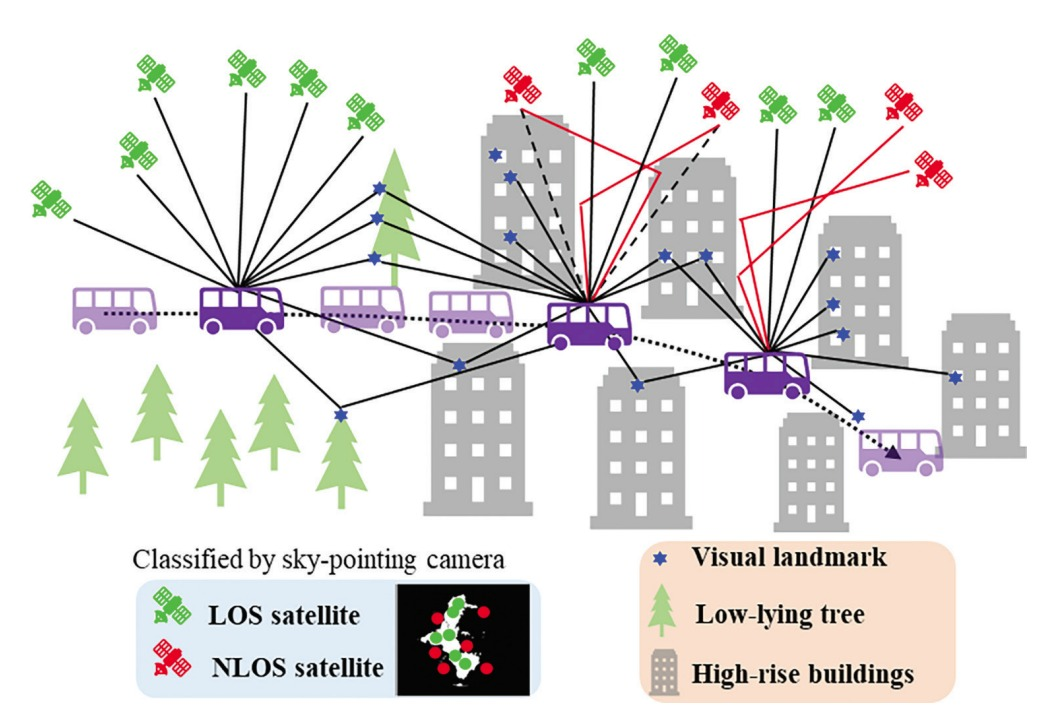
\includegraphics[width=0.8\textwidth]{images/gnss_signal.jpg}
    \caption{GNSS signal classification with LOS/NLOS satellites and visual landmarks in urban environments \cite{imgref1}.}
    \label{fig:gnss}
\end{figure}

The loss or degradation of GPS signals severely affects UAV navigation performance, leading to inaccurate positioning, trajectory deviations, and potential mission failure. These limitations prevent UAVs from operating autonomously in many real-world environments where GPS is unreliable or unavailable. Therefore, there is a critical need for reliable onboard localization methods that enable autonomous UAV navigation in GPS-denied environments without relying on satellite-based positioning systems.

\subsection{Research Objectives}

The main objective of this project is to develop and improve a robust localization system to enable autonomous UAV navigation in GPS-denied environments using onboard sensing technologies.

The specific objectives of this research are as follows:

\begin{itemize}

\item Study and analyze existing localization methods for UAV navigation in GPS-denied environments.

\item Evaluate alternative onboard localization approaches and select a suitable method for autonomous UAV operation.

\item Analyze existing Visual SLAM and Visual-Inertial SLAM algorithms and select an appropriate model for implementation.

\item Implement the selected localization model on a UAV platform and evaluate its baseline localization performance.

\item Identify limitations and performance constraints of the implemented system under real-world operating conditions.

\item Develop and integrate deep learning-based improvements to enhance localization robustness and accuracy.

\item Evaluate and compare the performance of the improved system against the baseline implementation.

\end{itemize}

\subsection{Purpose and Scope of the Project}

This project focuses on the development and evaluation of a robust onboard localization system for autonomous UAV operation in GPS-denied environments. The scope of the project includes the analysis of existing localization methods, selection and implementation of a suitable Visual-Inertial SLAM model, and evaluation of its performance on a UAV platform.

Furthermore, this project aims to investigate the limitations of the selected model and explore deep learning-based techniques to improve localization robustness and accuracy. The final outcome is a UAV system capable of reliable autonomous navigation using onboard visual and inertial sensing without dependence on GPS, enabling operation in challenging and previously inaccessible environments.